 % Sombras en seguidores de doble eje con PSTricks
 % Copyright (C) 2010 Oscar Perpiñán Lamigueiro
 %
 % This program is free software; you can redistribute it and/or
 % modify it under the terms of the GNU General Public License
 % as published by the Free Software Foundation; either version 2
 % of the License, or (at your option) any later version.
 %
 % This program is distributed in the hope that it will be useful,
 % but WITHOUT ANY WARRANTY; without even the implied warranty of
 % MERCHANTABILITY or FITNESS FOR A PARTICULAR PURPOSE.  See the
 % GNU General Public License for more details.
 %
 % You should have received a copy of the GNU General Public License
 % along with this program; if not, write to the Free Software
 % Foundation, Inc., 59 Temple Place - Suite 330, Boston, MA  02111-1307, USA.
\usepackage[T1]{fontenc}
\usepackage[utf8]{inputenc}
\usepackage[a4paper]{geometry}
\geometry{verbose,tmargin=2.5cm,bmargin=2.5cm,lmargin=2.5cm,rmargin=2.5cm}
\pagestyle{Ruled}
\usepackage{array}
\usepackage{verbatim}
\usepackage{prettyref}
\usepackage{booktabs}
\usepackage{textcomp}
\usepackage{url}
\usepackage{amsmath}
\usepackage{chemarr}%flechas para reacciones químicas (SFER.tex)
\usepackage{graphicx}
\usepackage{amssymb}
\usepackage{nomencl}
\usepackage[usenames,dvipsnames]{xcolor}

% the following is useful when we have the old nomencl.sty package
% \providecommand{\printnomenclature}{\printglossary}
% \providecommand{\makenomenclature}{\makeglossary}
\makenomenclature

\usepackage[caption=false]{subfig}
%Configuración de los caption
%\PassOptionsToPackage{caption=false}{subfig}%Evita que el paquete subfig lo descabale todo
\captiontitlefont{\itshape}
\captionnamefont{\scshape}
%\captionstyle{\centering}
\hangcaption


\usepackage[spanish]{babel}
\addto\shorthandsspanish{\spanishdeactivate{~<>}}


\usepackage[emulate=units]{siunitx}
\sisetup{per=fraction, fraction=nice, decimalsymbol=comma}
%\usepackage{lscape}
\usepackage{mathpazo}%Letra palatino con fuentes para matemáticas
\usepackage{flafter}%obliga a que los flotantes aparezcan después de su referencia
\usepackage{memhfixc}
\usepackage{mempatch}


\raggedbottom
\sloppybottom
\clubpenalty=10000
\widowpenalty=10000

%\raggedbottomsection
\feetbelowfloat


\usepackage[citestyle=authoryear, backend=bibtex, bibstyle=authoryear, doi=true, url=true]{biblatex}
\addbibresource{../biblio.bib}
\let\cite\parencite

\renewcommand{\bibsection}{%
	\chapter*{\bibname}
	\bibmark
	\phantomsection
	\addcontentsline{toc}{chapter}{\bibname}
	\prebibhook}
% \renewcommand{\bbltechreport}{Informe T\'ecnico}

\usepackage{hyperref}


\hypersetup{
    bookmarks=true,         % show bookmarks bar?
    unicode=true,          % non-Latin characters in Acrobat’s bookmarks
    bookmarksnumbered=false,
    bookmarksopen=false,
    breaklinks=true,
    backref=true,
    pdftoolbar=true,        % show Acrobat’s toolbar?
    pdfmenubar=true,        % show Acrobat’s menu?
    pdffitwindow=false,     % window fit to page when opened
    pdfstartview={FitH},    % fits the width of the page to the window
    pdftitle={Energía Solar Fotovoltaica},    % title
    pdfauthor={Oscar Perpiñán Lamigueiro},     % author
    pdfsubject={Energia Solar Fotovoltaica},   % subject of the document
    pdfcreator={AucTeX/Emacs},   % creator of the document
    pdfproducer={LaTeX}, % producer of the document
    pdfkeywords={radiación solar, energía solar fotovoltaica, energías
    renovables}, % list of keywords
    pdfnewwindow=true,      % links in new window
    pdfborder={0 0 0},
    colorlinks=true,       % false: boxed links; true: colored links
    linkcolor=Brown,          % color of internal links
    citecolor=BrickRed,        % color of links to bibliography
    filecolor=black,      % color of file links
    urlcolor=Blue           % color of external links 
}
	

\DeclareSIUnit\kWh{kWh}
\DeclareSIUnit\Wh{Wh}
\DeclareSIUnit\Wp{Wp}
\DeclareSIUnit\kWp{kWp}
\DeclareSIUnit\amperehour{Ah}
\DeclareSIUnit\celula{celula}

%\spanishdecimal{.} %Para que no lo sustituya automáticamente por comas
\addto\captionsspanish{%
\def\tablename{Tabla}%
\def\listtablename{\'Indice de tablas}}

\renewcommand\nomname{Nomenclatura}
\def\nompreamble{\addcontentsline{toc}{chapter}{\nomname}\markboth{\nomname}{\nomname}}


%\@addtoreset{equation}{section}
%\renewcommand{\theequation}{\thesection.\arabic{equation}}
%\numberwithin{equation}{section}
%\@addtoreset{table}{section}
%\renewcommand{\thetable}{\thesection.\arabic{table}}
%\numberwithin{table}{section}
%\@addtoreset{figure}{section}
%\renewcommand{\thefigure}{\thesection.\arabic{figure}}
%\numberwithin{figure}{section}


%\declarebtxcommands{spanish}{%
 % \def\btxphdthesis#1{\protect\foreignlanguage{spanish}{Tesis Doctoral}}%
%}
%\setbibliographyfont{lastname}{\scshape}%Pone los autores en Small Caps



%Configuración de MEMOIR
%%Pone la fecha en SMALL CAPS y hacia la derecha
%%pagina 60 de memman.pdf
\pretitle{\vfill \begin{flushright} \bfseries \scshape \HUGE \color{BrickRed}}
\posttitle{\par\end{flushright}}

\preauthor{\begin{flushright} \large \scshape}
\postauthor{\par\end{flushright}}

%\date{}
\predate{\vfill \begin{flushright}\large\scshape}
\postdate{\par\end{flushright}\vfill}

\setsecnumdepth{subsection}


% \definecolor{ared}{rgb}{.647,.129,.149}
% \renewcommand{\colorchapnum}{\color{ared}}
% \renewcommand{\colorchaptitle}{\color{ared}}
% \chapterstyle{pedersen}
\chapterstyle{ger}

\setlength{\afterchapskip}{35pt}
\maxtocdepth{section}

%\setcounter{topnumber}{3}
%\setcounter{bottomnumber}{2}
%\setcounter{totalnumber}{4}
\renewcommand{\topfraction}{0.85}
\renewcommand{\bottomfraction}{0.5}
\renewcommand{\textfraction}{0.15}
\renewcommand{\floatpagefraction}{0.7}


%Centra las figuras en los flotantes y los enmarca
\makeatletter
\renewenvironment{figure}[1][]{%
     	\@float{figure}%
		%\begin{framed}    
		\precaption{\rule{\linewidth}{0.4pt}\par}%En las figuras el caption va debajo
		%\hrule\vspace{\onelineskip}
		\centering
		  }{%
		%\end{framed}
		%\postcaption{\rule{\linewidth}{0.4pt}}
		%\vspace{\onelineskip}\hrule
    	\end@float	
}
\makeatother

\makeatletter
\renewenvironment{table}[1][]{%
      	\@float{table}%
		%\begin{framed}    
		\postcaption{\rule{\linewidth}{0.4pt}\par}%En las tablas el caption va encima
		\centering
		  }{%
		%\end{framed}
    	\end@float	
}
\makeatother


\renewcommand{\textfloatsep}{10pt}%Espacio entre el flotante y el texto

%backgroung image
\usepackage{eso-pic} 

%http://stackoverflow.com/questions/240097/how-to-create-a-background-image-on-titlepage-with-latex
\newcommand\BackgroundPic{
  \put(350,-150){
    \parbox[b][0.5\paperheight]{0.5\paperwidth}{%
      \includegraphics[scale=0.5]{../figs/johnny_automatic_old_sun}%
}}}

\newcommand\BackgroundPicLight{
  \put(350,-150){
    \parbox[b][0.5\paperheight]{0.5\paperwidth}{%
 %     \vfill 
%\centering
      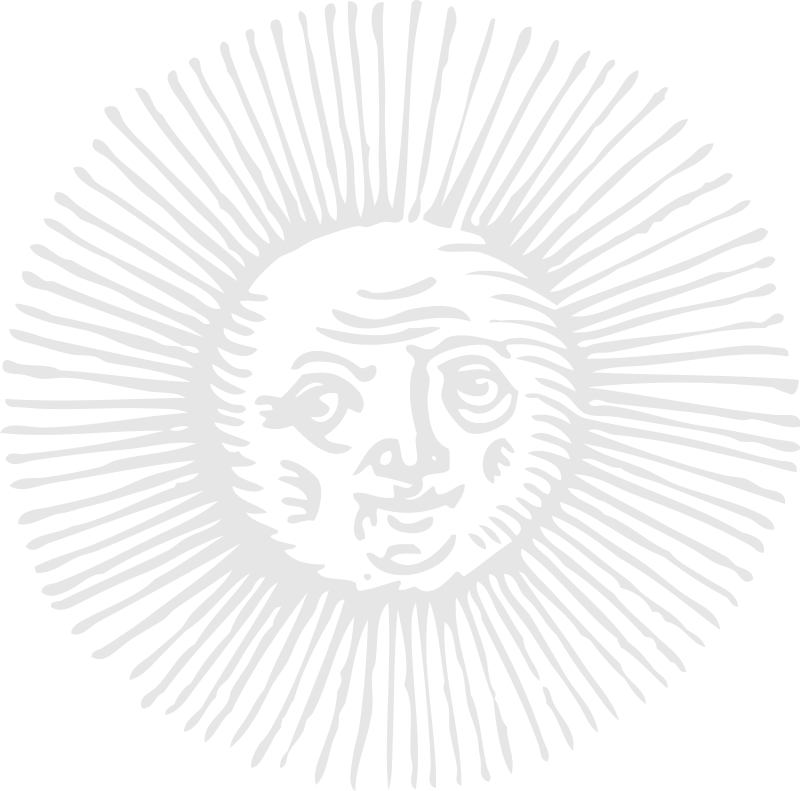
\includegraphics[scale=0.5]{../figs/johnny_automatic_old_sun_light}%
%\vfill
}}}


\begin{document}
\def\Rectangle(#1,#2)(#3,#4){
newpath
#1 #2 moveto
#3 #2 lineto
#3 #4 lineto
#1 #4 lineto
 closepath }

\def\cercle(#1,#2)#3{%
newpath
 #1 #2 #3 0 360 arc
closepath }

\def\ARC(#1,#2)#3#4#5{%
newpath
 #1 #2 #3 #4 #5 arc }

\def\ARCN(#1,#2)#3#4#5{%
newpath
 #1 #2 #3 #4 #5 arcn }

\def\Sombra(#1,#2){%
        \NodeIIItoIID[origine=#1 #2 0,normale=90 \BETA neg add \ALFA](-3,-1){s1}
        %\psdot(s1)
        \NodeIIItoIID[origine=#1 #2 0,normale=90 \BETA neg add \ALFA](3,-1){s2}
        %\psdot(s2)
        \NodeIIItoIID[origine=\s 180 \ALFA add cos mul #1 add \s 180 \ALFA add sin mul #2 add 0,normale=90 \BETA neg add \ALFA](-3,-1){s3}
        %\psdot(s3)
        \NodeIIItoIID[origine=\s 180 \ALFA add cos mul #1 add \s 180 \ALFA add sin mul #2 add 0,normale=90 \BETA neg add \ALFA](3,-1){s4}
        %\psdot(s4)
        \pspolygon[linecolor=gray,fillstyle=solid,fillcolor=lightgray](s1)(s3)(s4)(s2)}
\psset{hatchwidth=0.02}


\def\rad{\Lns }
\def\radang{\rad 1.8 div }

\def\az{60 }%cuidado con los signos
\def\el{45 }
\def\BETA{90 -\el add }
\def\ALFA{\az }

\def\W{23 }
\def\L{10 }
\def\Lns{30 }
\def\Lew{50 }
\def\TANel{\el sin \el cos div }

\def\Sa{\L \BETA cos mul }
\def\Sb{\L \BETA sin mul \TANel div  } 
\def\s{\Sa \Sb add }

%\begin{center}
	\psset{unit=.5cm}
	\begin{pspicture}(-5,-6)(19,8)
		%\psframe(-5,-4)(19,8)
		\psset{THETA=10,PHI=20,Dobs=\Lew 2 mul,Decran=20,arrowsize=0.3}
		%\axesIIID(20,20,20)%
		%\planThreeDput[normale=90 0,linecolor=gray,fontscale=0.5](0,0,0){\Grille(-10,-8)(10,8)}
		\pnodeXYZ(0,0,0){O}
		\pnodeXYZ(0,0,\Lns){Z}
		\uput[90](Z){Zenith}%{$\vec{\mu}_c$}
		\pnodeSphericalCoor(\Lns 1.5 mul,0,0){X}
		\uput[180](X){South}%{$\vec{\mu}_h$}
		\pnodeSphericalCoor(\Lew 1.5 mul,90,0){Y}
		\uput[0](Y){East}%{$\vec{\mu}_\bot$}
		\psline{->}(O)(X)
		\psline{->}(O)(Y)
		\psline{->}(O)(Z)
		
		\pnodeXYZ(\Lns,0,0){Seg2}
		\pnodeXYZ(\Lns,\Lew,0){Seg3}
		\pnodeXYZ(0,\Lew,0){Seg4}
		\pnodeXYZ(0,-\Lew,0){Seg5}
		\pnodeXYZ(\Lns,-\Lew,0){Seg6}

		\pnodeXYZ(\Lns,\Lew 2 div,0){Lew}
		\pnodeXYZ(\Lns 2 div,\Lew,0){Lns}
		
		\pnodeSphericalCoor(\rad,\ALFA,90 \BETA neg add){V}
		\pnodeSphericalCoor(\rad 90 \BETA neg add cos mul,\ALFA,0){Vp}
		
		
		
		%\psline(A)(B)
		%\psline(B)(C)
		%\Sombra(0,0)
		%\Sombra(\Lns,0)
		%\Sombra(0,\Lew)
		%\Sombra(\Lns,\Lew)
		\psset{linestyle=solid,linewidth=.5pt,linecolor=gray,fillstyle=solid,fillcolor=lightgray}
		\planThreeDput[normale=90 \ALFA](0,0,0){\Rectangle(\W 2 div neg,0)(\W 2 div,\s)}
		\planThreeDput[normale=90 \ALFA,translation=\Lns 0 0]{\Rectangle(\W 2 div neg,0)(\W 2 div,\s)}
		\planThreeDput[normale=90 \ALFA,translation=0 \Lew 0]{\Rectangle(\W 2 div neg,0)(\W 2 div,\s)}
		\planThreeDput[normale=90 \ALFA,translation=\Lns \Lew 0]{\Rectangle(\W 2 div neg,0)(\W 2 div,\s)}
		\planThreeDput[normale=90 \ALFA,translation=0 -\Lew 0]{\Rectangle(\W 2 div neg,0)(\W 2 div,\s)}
		\planThreeDput[normale=90 \ALFA,translation=\Lns -\Lew 0]{\Rectangle(\W 2 div neg,0)(\W 2 div,\s)}
		
		
		\psset{linestyle=solid,linewidth=1pt,linecolor=black,fillstyle=solid,fillcolor=blue!30}
		\planThreeDput[normale=90 \BETA neg add \ALFA](0,0,0){\Rectangle(\W 2 div neg,0)(\W 2 div,\L)}
		\planThreeDput[normale=90 \BETA neg add \ALFA,translation=\Lns 0 0]{\Rectangle(\W 2 div neg,0)(\W 2 div,\L)}
		\planThreeDput[normale=90 \BETA neg add \ALFA,translation=0 \Lew 0]{\Rectangle(\W 2 div neg,0)(\W 2 div,\L)}
		\planThreeDput[normale=90 \BETA neg add \ALFA,translation=\Lns \Lew 0]{\Rectangle(\W 2 div neg,0)(\W 2 div,\L)}
		\planThreeDput[normale=90 \BETA neg add \ALFA,translation=0 -\Lew 0]{\Rectangle(\W 2 div neg,0)(\W 2 div,\L)}
		\planThreeDput[normale=90 \BETA neg add \ALFA,translation=\Lns -\Lew 0]{\Rectangle(\W 2 div neg,0)(\W 2 div,\L)}
		
		\psset{fillstyle=none,linecolor=black,linewidth=.4pt,linestyle=dashed}
		\planThreeDput[normale=0 270 \ALFA add,]{\ARC(0,0){\radang}{90 \BETA neg add}{90}}
		\planThreeDput[normale=90 0]{\ARC(0,0){\radang}{-90}{-90 \az add}}
		\pnodeSphericalCoor(\radang,\ALFA,90 \BETA add 2 div){BETA}
		%\pnodeXYZ(\radang \el 2 div cos \az cos mul mul,\radang \el 2 div cos \az sin mul mul,\radang \el 2 div sin mul){phi}
		\uput{0pt}[45](BETA){$\beta$}
		\pnodeSphericalCoor(\radang,\ALFA 2 div,0){ALFA}
		%\pnodeXYZ(\radang \az 2 div cos mul,\radang \az 2 div sin mul,0){theta}
		\uput{5pt}[225](ALFA){$\alpha$}
		
		
		\psset{linestyle=dashed,linewidth=.5pt,linecolor=gray,arrows=|-|,arrowsize=10pt}
		\psline(O)(Seg2)
		\psline(O)(Seg4)
		\psline(Seg3)(Seg4)
		\psline(Seg3)(Seg2)
                \psline(O)(Seg5)
                \psline(Seg5)(Seg6)
                \psline(Seg2)(Seg6)
		\uput{10pt}[180](Lew){$L_{ew}$}%{$L_{eo}$}
		\uput{3pt}[90](Lns){$L_{ns}$}
		
		\psset{linestyle=solid,linecolor=black,linewidth=.4pt,arrowsize=4pt}
		\psline{->}(O)(V)
		\psline{->}(O)(Vp)
		\psset{linestyle=dashed,linewidth=.2pt}
		\psline(Vp)(V)
		
		\uput[0](V){$\vec{\mu}_{2x}$}
	\end{pspicture}
%\end{center}
\end{document}